\documentclass{article}
\usepackage{graphicx}
\usepackage[margin=1.5cm]{geometry}
\usepackage{amsmath}

\begin{document}

\title{Tuesday Reading Assessment: Chapters 3, 4-1 and 4-2}
\author{Prof. Jordan C. Hanson}

\maketitle

\section{Boolean Algebra}

\begin{enumerate}
\item Let the conjugate of a boolean input $A$ be $\bar{A}$.  The circuit equivalent of the conjugate is the action of the inverter, changing $0$ to $1$ and $1$ to $0$.  Further, recall that Boolean multiplication is equivalent to an AND gate, and addition is equivalent to an OR gate.  Write the truth table for the following boolean expression:
\begin{equation}
\bar{X} Y Z + X\bar{Y}Z + XY\bar{Z}
\end{equation}
\vspace{1cm}
\end{enumerate}

\section{Programmable Logic: The AND Array}

\begin{enumerate}
\item
\begin{figure}[ht]
\centering
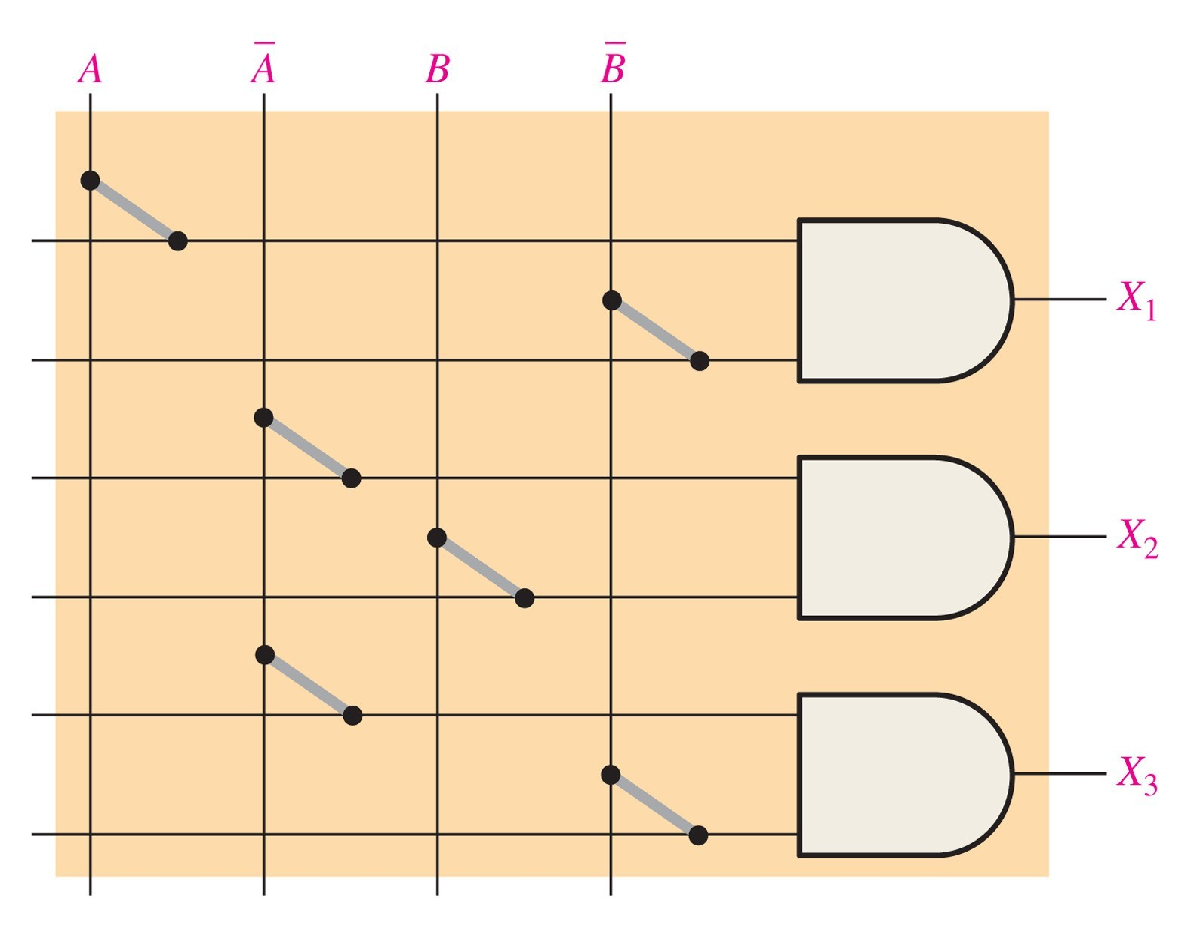
\includegraphics[width=0.25\textwidth]{figures/ANDArray.pdf}
\caption{\label{fig:array} An example of the AND array within the broader category of PLAs.}
\end{figure}
(a) What are the logical expressions for the AND array outputs in the PLA shown in Fig. \ref{fig:array}? (b) Draw new connections such that: $X_1 = \bar{A}B$, $X_2 = AB$, and $X_3 = A\bar{B}$.
\end{enumerate}

\section{Troubleshooting: Open and Closed Gates}

\begin{enumerate}
\item 
\begin{figure}[hb]
\centering
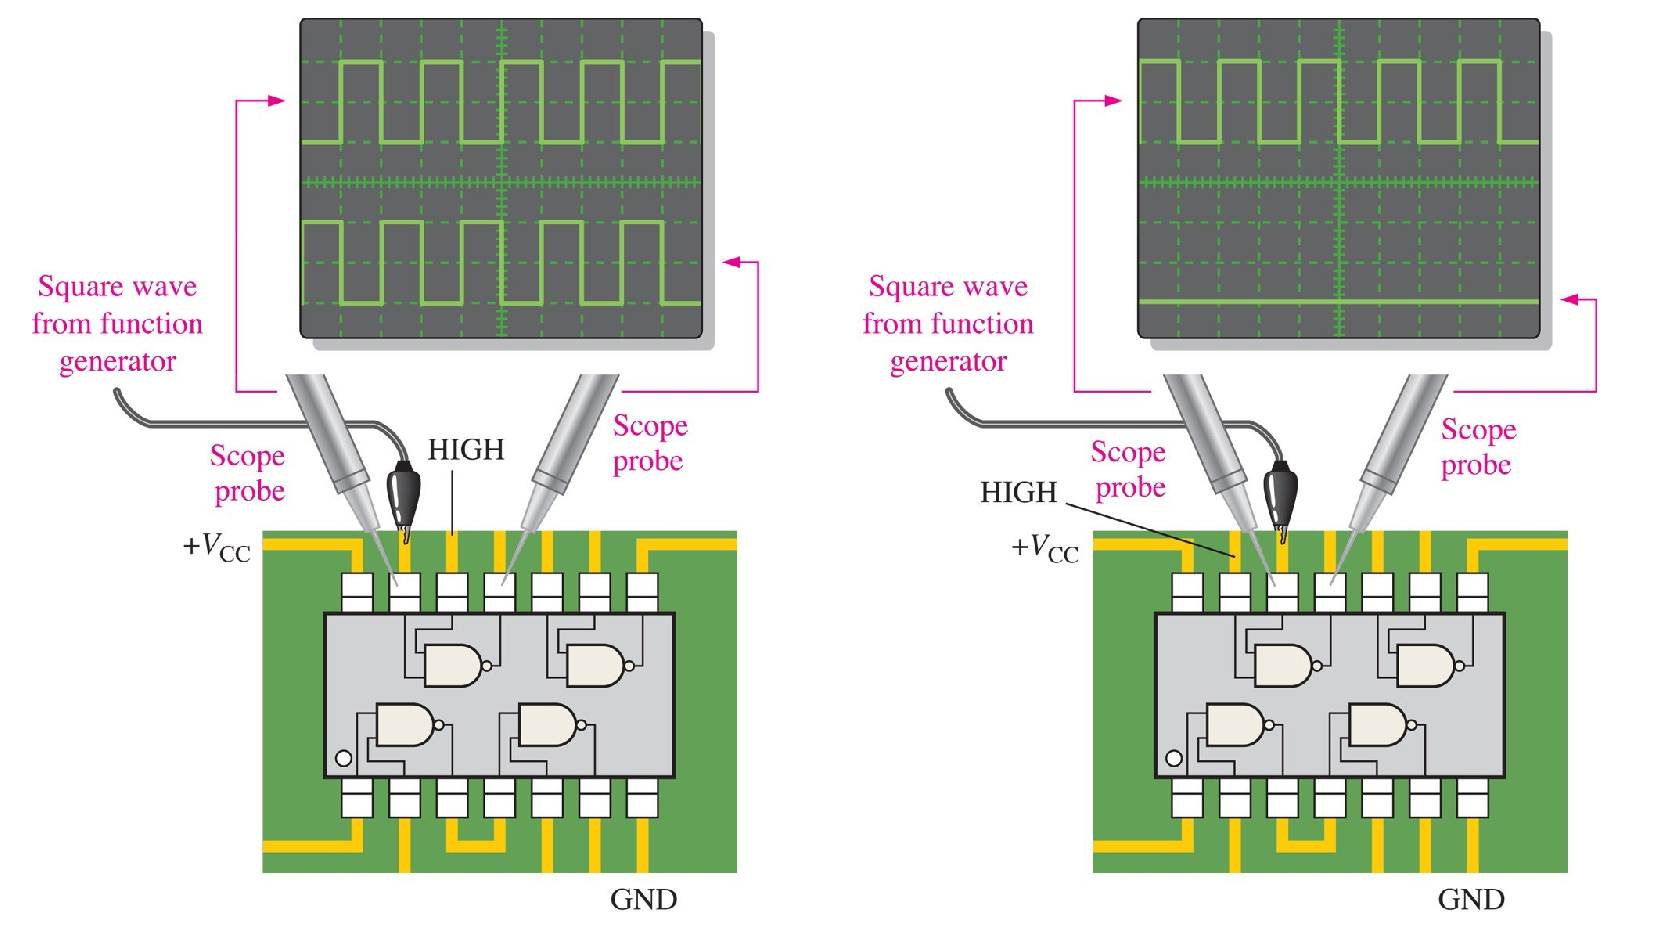
\includegraphics[width=0.45\textwidth]{figures/troubleShoot.pdf}
\caption{\label{fig:troubleshoot} An example of probing a suspect gate with pulsed signal on one input, and HIGH on the other.}
\end{figure}
Which input on the NAND gate pictured in the experiment in Fig. \ref{fig:troubleshoot} is faulty?  What is its level (0 or 1)?
\end{enumerate}

\end{document}
